\chapter{Architecture}

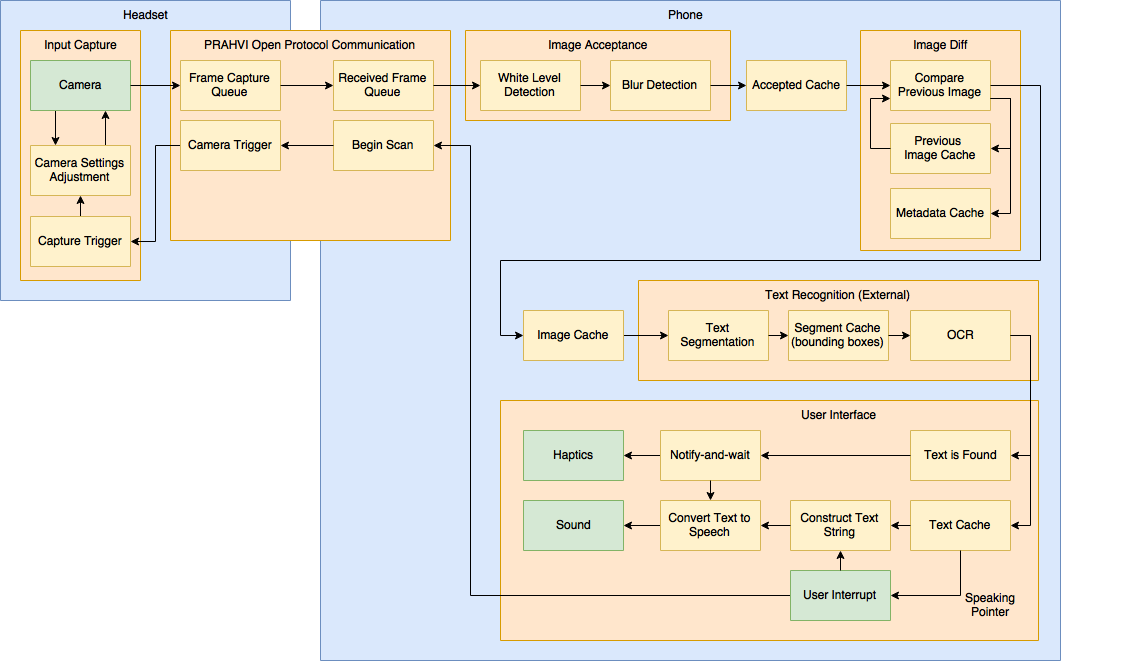
\includegraphics[scale = 0.4]{PRAHVI-Block.png}

\section{Activity Diagram}
Figure~\ref{activityDiagram} is the high level data-flow architecture of the system that shows the flow of actions of the user. Input is first received by the system to begin capturing an image of the user's immediate gaze, or view, in front of them. The system then evaluates the image and notifies the user if the image needs to be recaptured because it is too blurry or the text is illegible. If the image passes this evaluation, the system then translates the image into text and generates a summary for the user. This summary is then read aloud to the user. If the user takes no action at this point, the system proceeds to reading the entire text article. This architecture was chosen because there are constant inputs received by the system, and the inputs in general goes through the same route within the system. The data-flow architecture also has build-in concurrency, which can speeds up the process, especially the platform in which the product is embedded.

\begin{figure}
	\centering
    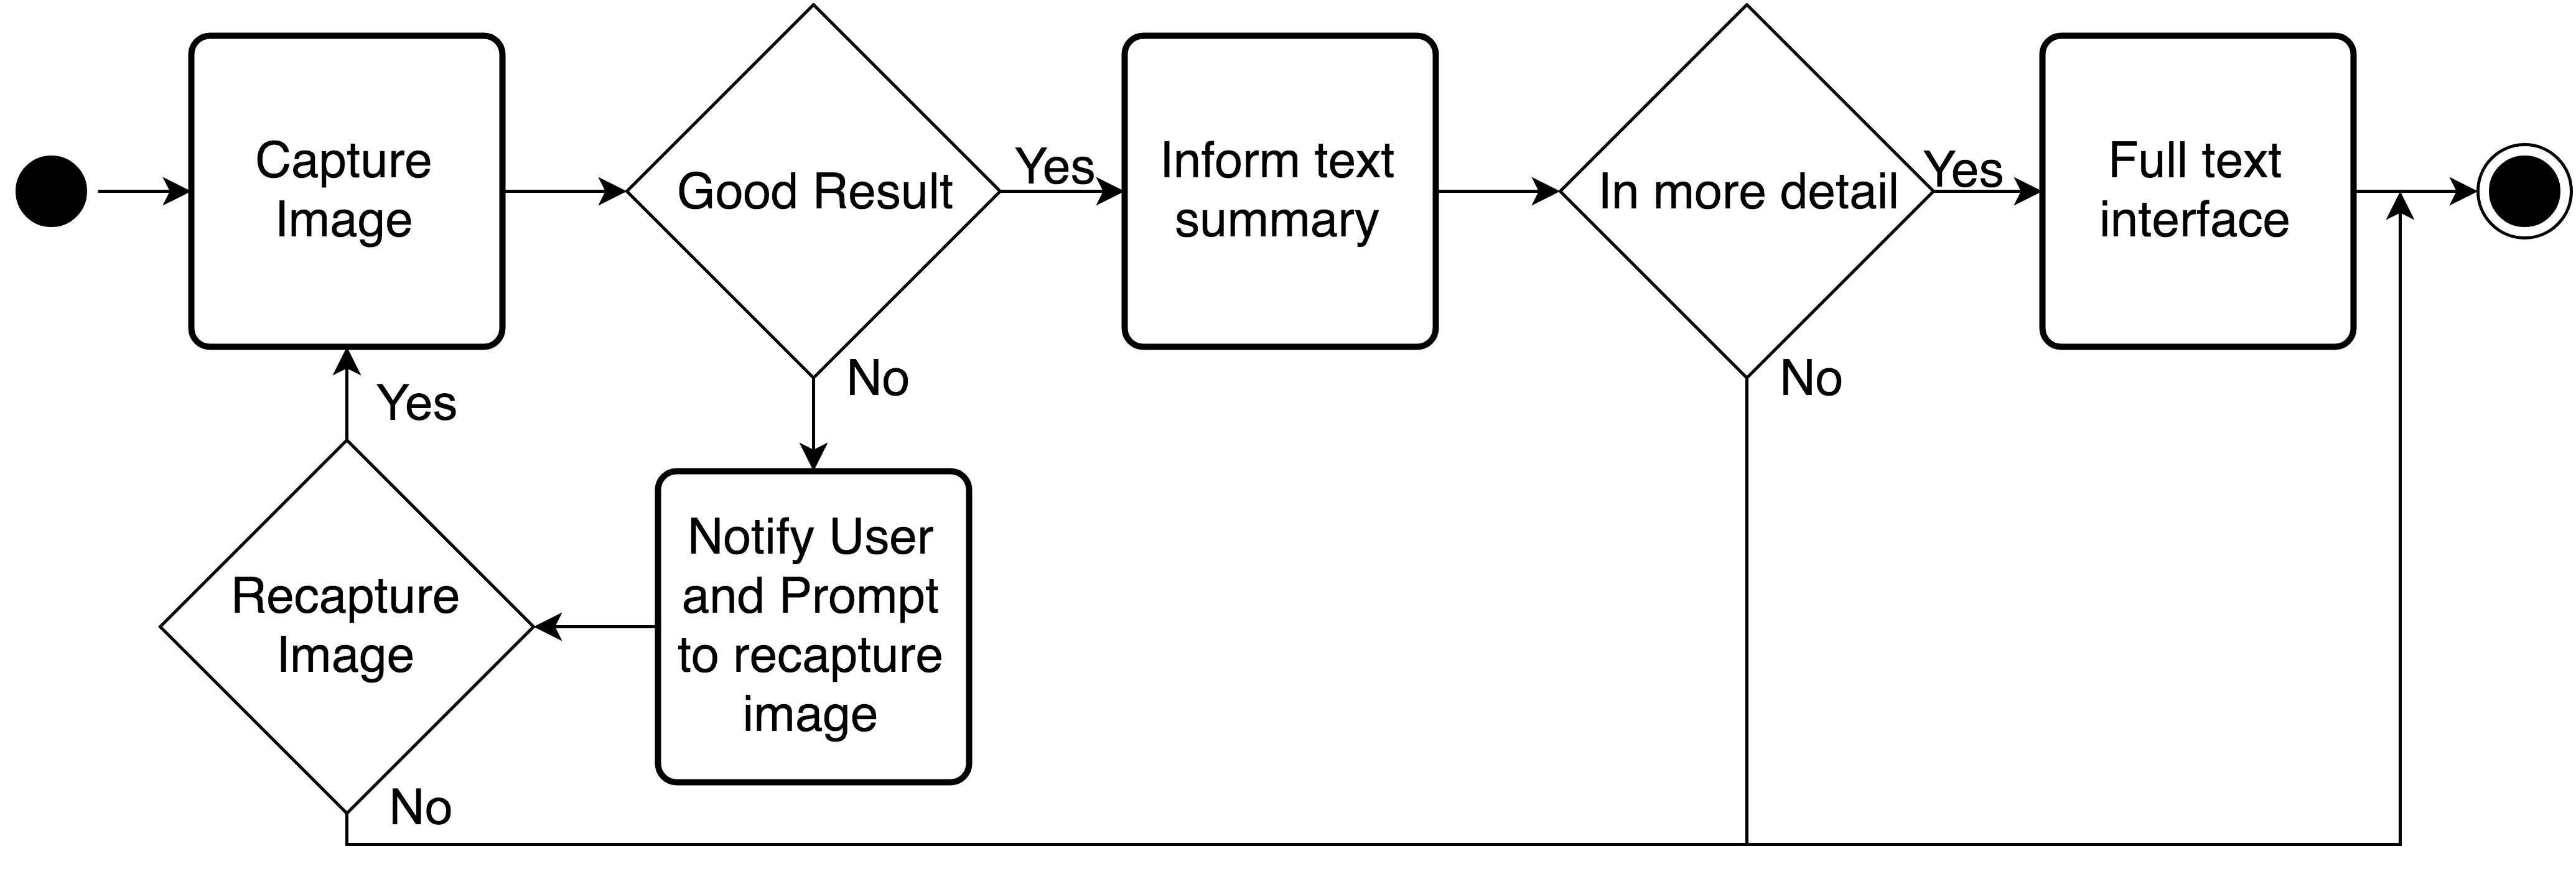
\includegraphics[scale = 0.105]{Activity_H.png}%{activityDiagram.png}
    
    \caption{High Level View}
	\label{activityDiagram}
\end{figure}

\section{Hardware}
The most visible component of PRAHVI is its wearable headset device that attaches to a typical pair of glasses or can be manufactured as a single assembly. The headset (shown in appendix \ref{headsetPic}) is comprised of a Raspberry Pi Zero board coupled with a standard Raspberry Pi Camera. The Raspberry Pi Zero was chosen for its low power consumption, small footprint, and its UNIX-based operating system allows for wide application flexibility. This means that the Raspberry Pi Zero allows us to cut down on the device's size and weight while creating an extensible application platform. Its main shortcoming, processor speed, is mitigated by the fact we use a smartphone and external server to process the images. The Raspberry Pi Camera is a module comprised of a breakout board and a 5.0 megapixel smartphone camera. The cable used to connect the camera to the Raspberry Pi Zero is a standard accessory cable used by many third-party accessories. The modular nature of these parts allows for future expansion and easy repairs for the user and for other developers. 

When the device is connected to the user's smartphone and the accompanying app is opened, PRAHVI powers up and immediately begins communicating with the smartphone. Once the initial setup is completed, the headset waits for a trigger from the user to begin capturing images of the user's surroundings. Once this is triggered, the camera begins capturing a set of images which are added to a frame capture queue and used to adjust the camera settings, such as white balance and exposure, to achieve an optimal capture. An image sample is then served over the bridge created using the PRAHVI Open Protocol back to the smartphone. PRAHVI Open Protocol, or "POP," is a socket-oriented connection protocol based on the open source Bonjour networking standard.\footnote{https://developer.apple.com/bonjour/} Although the protocol is implemented for iOS and Python for this product, the protocol can be implemented on any platform or system that supports network sockets. These technologies and systems were ultimately employed to make using PRAHVI, from the moment the user connects the device, to the point the user requests a translation, as seamless and intuitive as possible from an ergonomics standpoint.

\begin{figure}
	\centering
	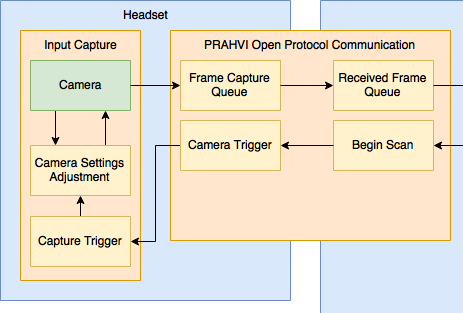
\includegraphics[scale = 0.6]{PRAHVI-HEADSET}
	\caption{Hardware Diagram}
	\label{headsetDiagram}
\end{figure}

\section{User Interface}
The user interface of PRAHVI is designed to operate entirely using haptic feedback and voice to simplify interaction and make text translation seamless. For this product, an app was written on the iOS platform to communicate with the headset device. The app (shown in \ref{uipicture}) is mainly comprised of a gesture pad that spans three fourths of the entire surface of the phone screen. Once the user connects the headset and opens the app, PRAHVI immediately connects to the app to set up the POP connection. When the user double taps the gesture area, the device begins scanning the environment, adjusting the camera parameters to find a set point that produces clear, usable images. From this queue, an image is selected using image acceptance algorithms and sent to the backend for translation. Once the translation is complete, the app stores the translated text into a cache and signals to the user a quick summary (see Text Summarization section for more information) of the text before proceeding with a full translation. Swiping the gesture area allows the user to navigate the text in realtime, with the smartphone providing haptic feedback. The user primarily interacts with the app to begin translation, proceed from the summary to the full translation, and navigate the translation. By using sound and touch as the primary modes of communication for the user interface, much of the interface could actually be removed, simplifying the experience for users.

\begin{figure}
	\centering
	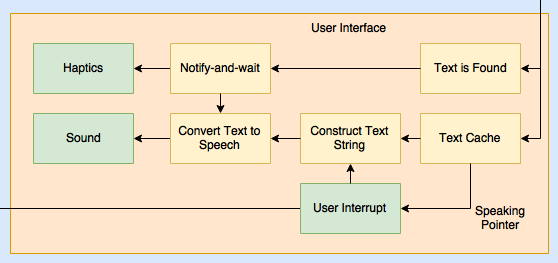
\includegraphics[scale = 0.6]{PRAHVI-UI.png}
	\caption{User Interface Diagram}
	\label{uiDiagram}
\end{figure}

\section{Backend}
The backend of PRAHVI is a flask web application. It exposes all the functionality related to the computer vision, optical character recognition, and text summary into a an easy web interface for our iPhone application to use.

The interface of the backend is a simple set of HTTP endpoints which are summarized as follows:

\begin{table}[]
\centering
\caption{PRAHVI API Endpoints}
\label{PRAHVI_API_endpoints}
\begin{tabular}{|l|l|l|l|l|}
\hline
\multicolumn{1}{|c|}{\textbf{Endpoint}} & \multicolumn{1}{c|}{\textbf{Input}}                                                   & \multicolumn{1}{c|}{\textbf{Output}}                                                                       & \multicolumn{1}{c|}{\textbf{\begin{tabular}[c]{@{}c@{}}HTTP\\ METHOD\end{tabular}}} & \multicolumn{1}{c|}{\textbf{Description}}                                                                                        \\ \hline
/api/v1/image/ocr3                      & File: Image                                                                           & \begin{tabular}[c]{@{}l@{}}JSON: \\ \{ result:\\    string \}\end{tabular}                                 & POST                                                                                & \begin{tabular}[c]{@{}l@{}}PRAHVI's image to text\\ algorithm using tesseract 3\end{tabular}                                     \\ \hline
/api/v1/image/ocr4                      & File: Image                                                                           & \begin{tabular}[c]{@{}l@{}}JSON: \\ \{ result:\\    string \}\end{tabular}                                 & POST                                                                                & \begin{tabular}[c]{@{}l@{}}PRAHVI's image to text\\ algorithm using tesseract 4\end{tabular}                                     \\ \hline
/api/v1/text/tfidf                      & String                                                                                & \begin{tabular}[c]{@{}l@{}}JSON:\\ \{result: \\    \{ term:\\       score, \\       ... \} \}\end{tabular} & POST                                                                                & \begin{tabular}[c]{@{}l@{}}Takes in a document string \\ and outputs the scores of \\ all the terms in the document\end{tabular} \\ \hline
/api/v1/text/compare                    & \begin{tabular}[c]{@{}l@{}}JSON: \\ \{ text1: string,\\ text2: string \}\end{tabular} & \begin{tabular}[c]{@{}l@{}}JSON:\\ \{ result: \\    int{[}0, 1{]} \}\end{tabular}                          & POST                                                                                & \begin{tabular}[c]{@{}l@{}}Returns a score of how\\ similar the documents are\end{tabular}                                       \\ \hline
\end{tabular}
\end{table}



\begin{itemize}

\item Originally, all of the functionality listed above was implemented within the iPhone application, however due to the limited compute resources of the iPhone, PRAHVI's requirements were not being met. Image to text translation on average would take half a min, and the iPhone architecture was mangling some of the text results. For these reasons, these functionalities have been moved the backend end hosted on a server allows for a faster processing time as noted in our test bench. The server is a linux machine running an Intel(R) Core(TM) i7-4900MQ CPU @ 2.80GHz multi-core processor.

\end{itemize}

\section{System Flow}
Once the camera captures the image and sends the image to the smart phone, the image will pass through the pre-processing stage to detect whether the image will be processed or not, based on the blurriness of the image and the similarity of the current image and the previous image (see Image Pre-processing for more information). Once the image has passed the pre-processing stage, it is also processed for text, which is stored in the smart phone. Access to text is by string, and different lines are separated by the new line character that is the same as the document captured. The text is then output as audio feedback as decided by the user (see Figure ).



\section{Text Extraction}

\subsection{Image Pre-processing}
When the smart phone application receives the image, the image is then passed through 2 filters. The first filter detects the blurriness of the image. If the image is blurred, the phone will reject the image because it is hard to extract useful information from a blurred imaged. If the image passed the blurriness test, it will then be used to compare to the previous detected image for similarity. If the image is similar (or the same), the image will also be rejected, because the information from the same document is stored in the device from the previous capture. These 2 filters help to improve the efficiency of the system and save time waited by the user.

\subsubsection{Blurriness Test}

To test for blurriness, variance of Laplacian \cite{PechPacheco} is used. The image is treated as a 2-dimensional matrix (after grayscaled), and convolve it with the 3x3 Laplacian kernel (see Figure~\ref{laplacianKernel}). The variance of Laplacian is the variance of the response. The variance of Laplacian of the image is then compared to a threshold value (the threshold value used for this system is 50). If the variance of Laplacian of the image is lower than the threshold, then the image is blurred, otherwise, it is not.
\begin{figure}
	\centering
    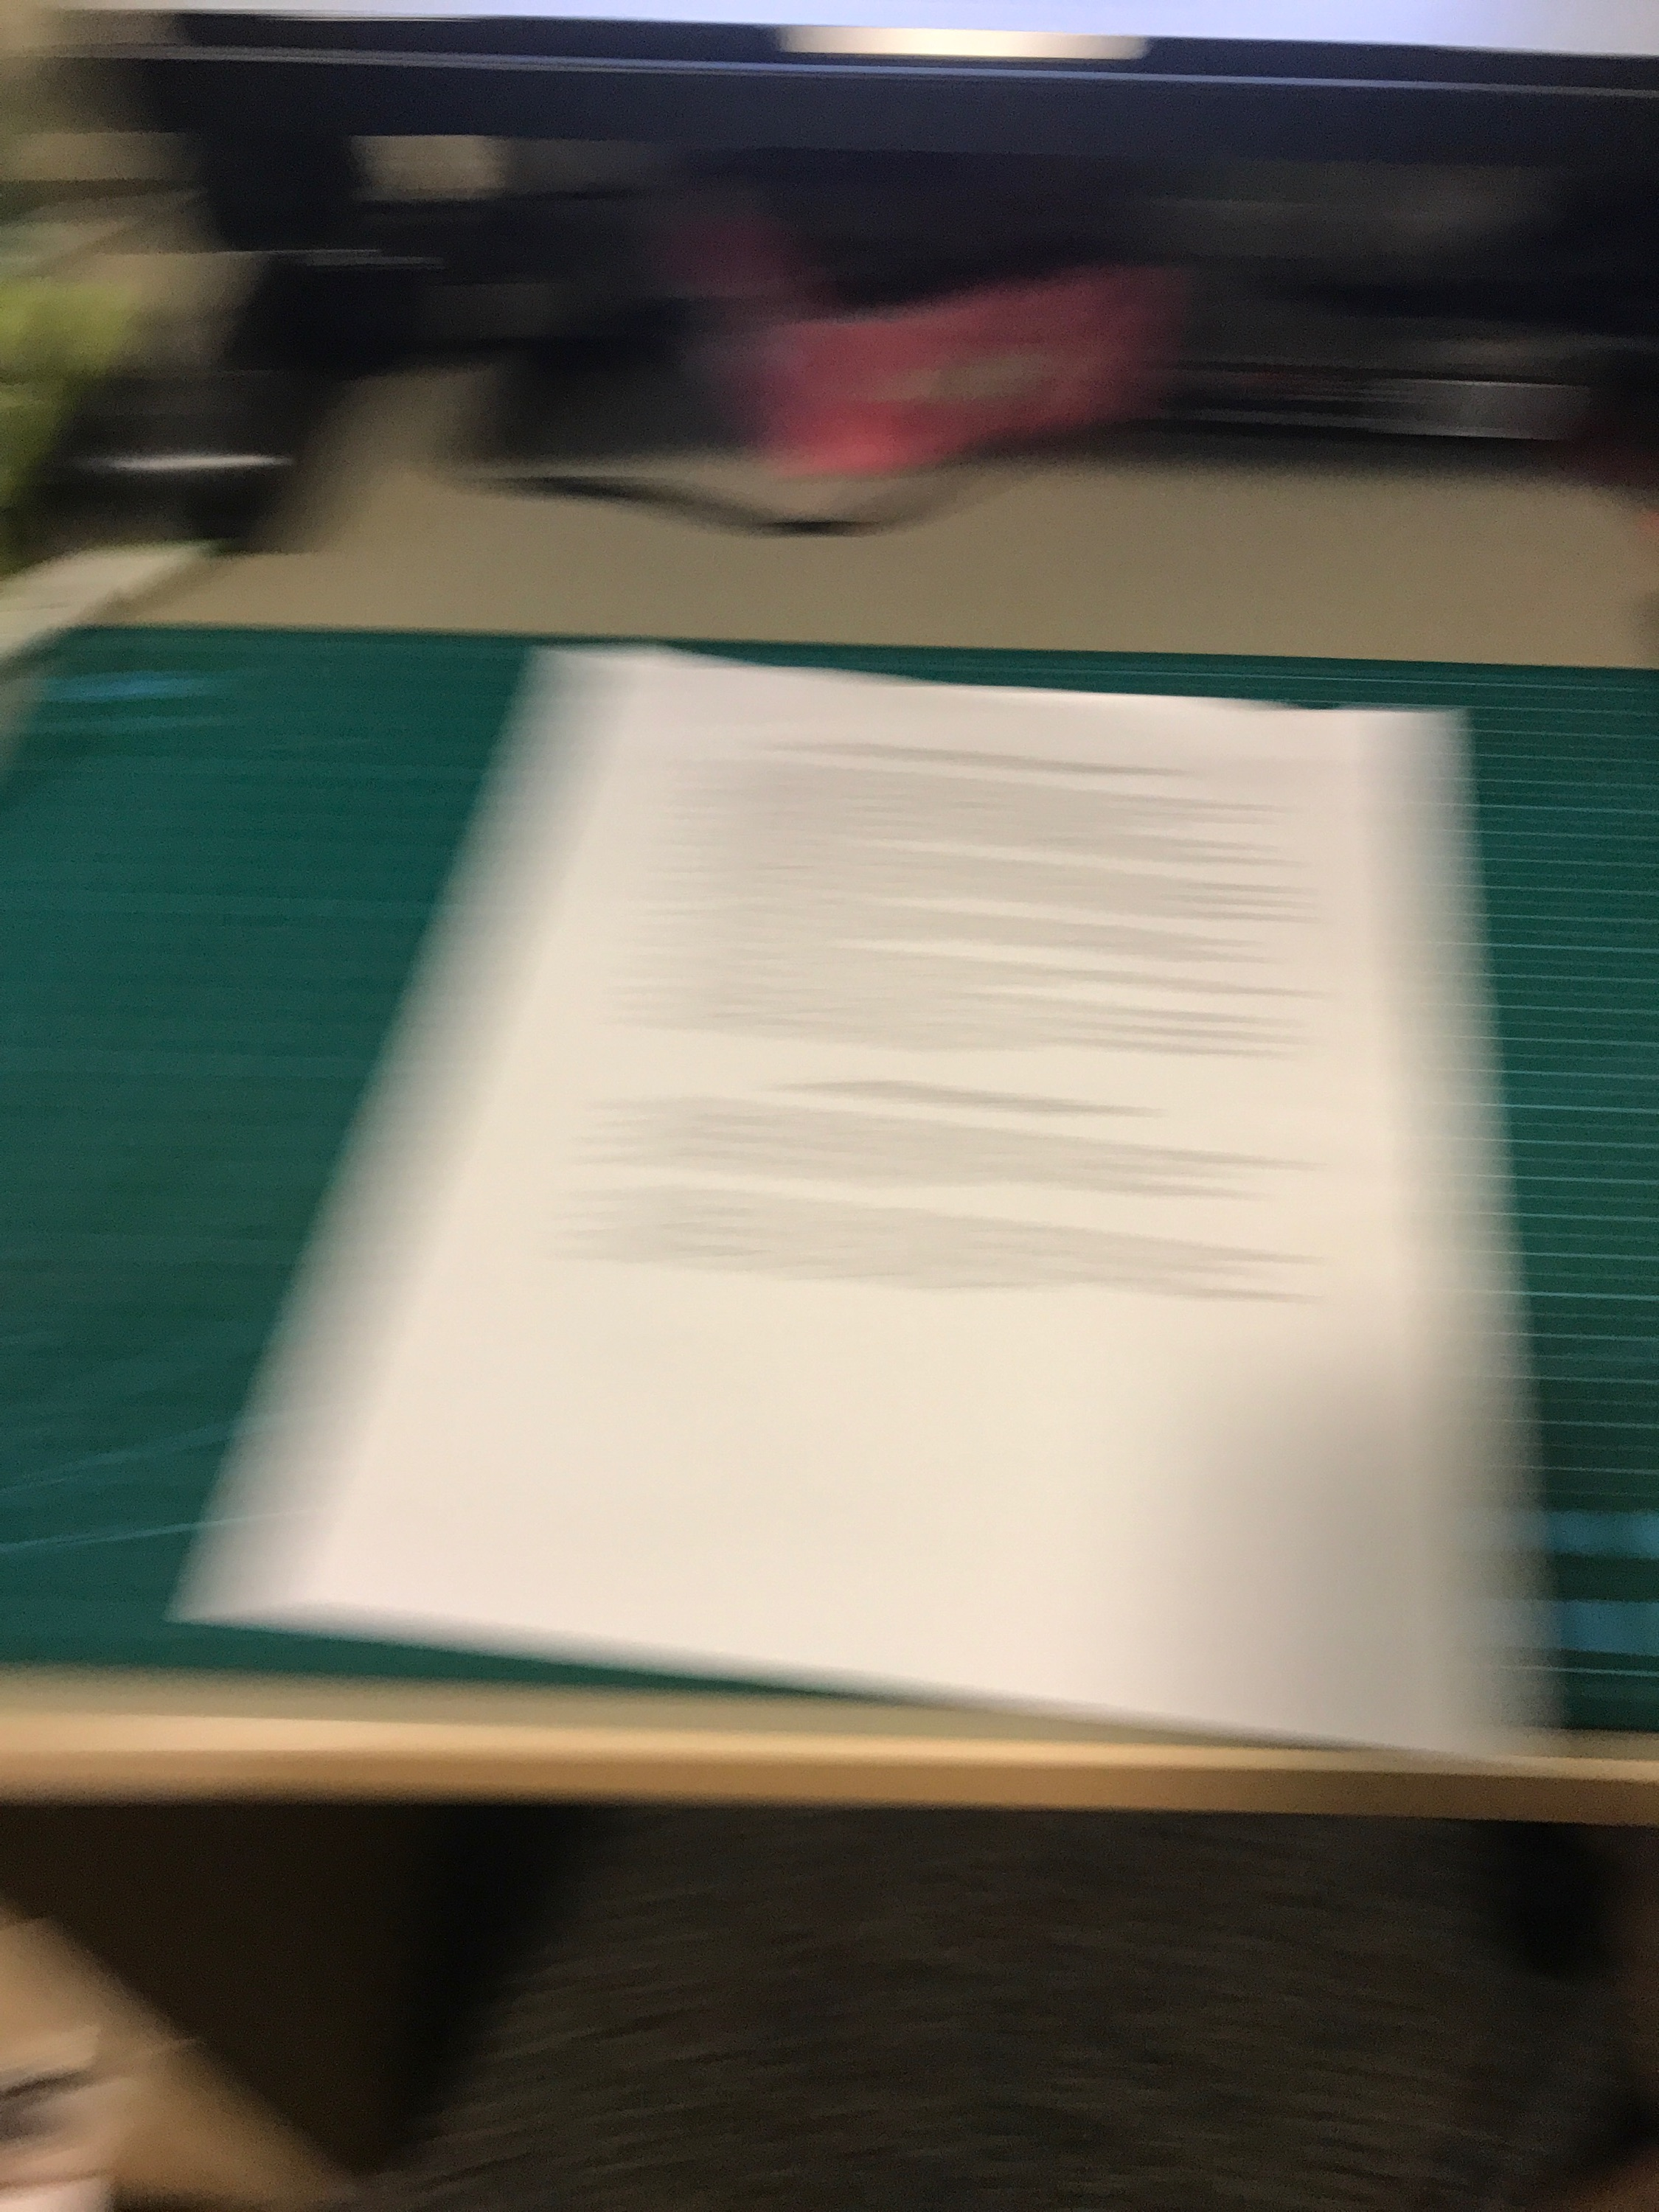
\includegraphics[scale = 0.075]{blur.jpg}
    
    \caption{Blurred image}
	\label{blurredImage}
\end{figure}

\begin{figure}
	\centering
    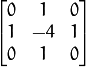
\includegraphics[scale = 0.5]{laplacian_kernel.png}
    
    \caption{The Laplacian kernel}
	\label{laplacianKernel}
\end{figure}

\subsubsection{Similarity Test}
The similarity test uses the accelerated-KAZE (AKAZE) local features matching \cite{akaze}.~The AKAZE local features matching returns a list of matches between the two images. We consider the two image is similar if the number of good matches is above the threshold (the threshold value used for this system is 1000), then the images is said to be similar. In other words, if the two images have the numbers of good matches that is greater than the threshold value, it is said to be similar.

\begin{figure}
  \begin{subfigure}{\linewidth}
	  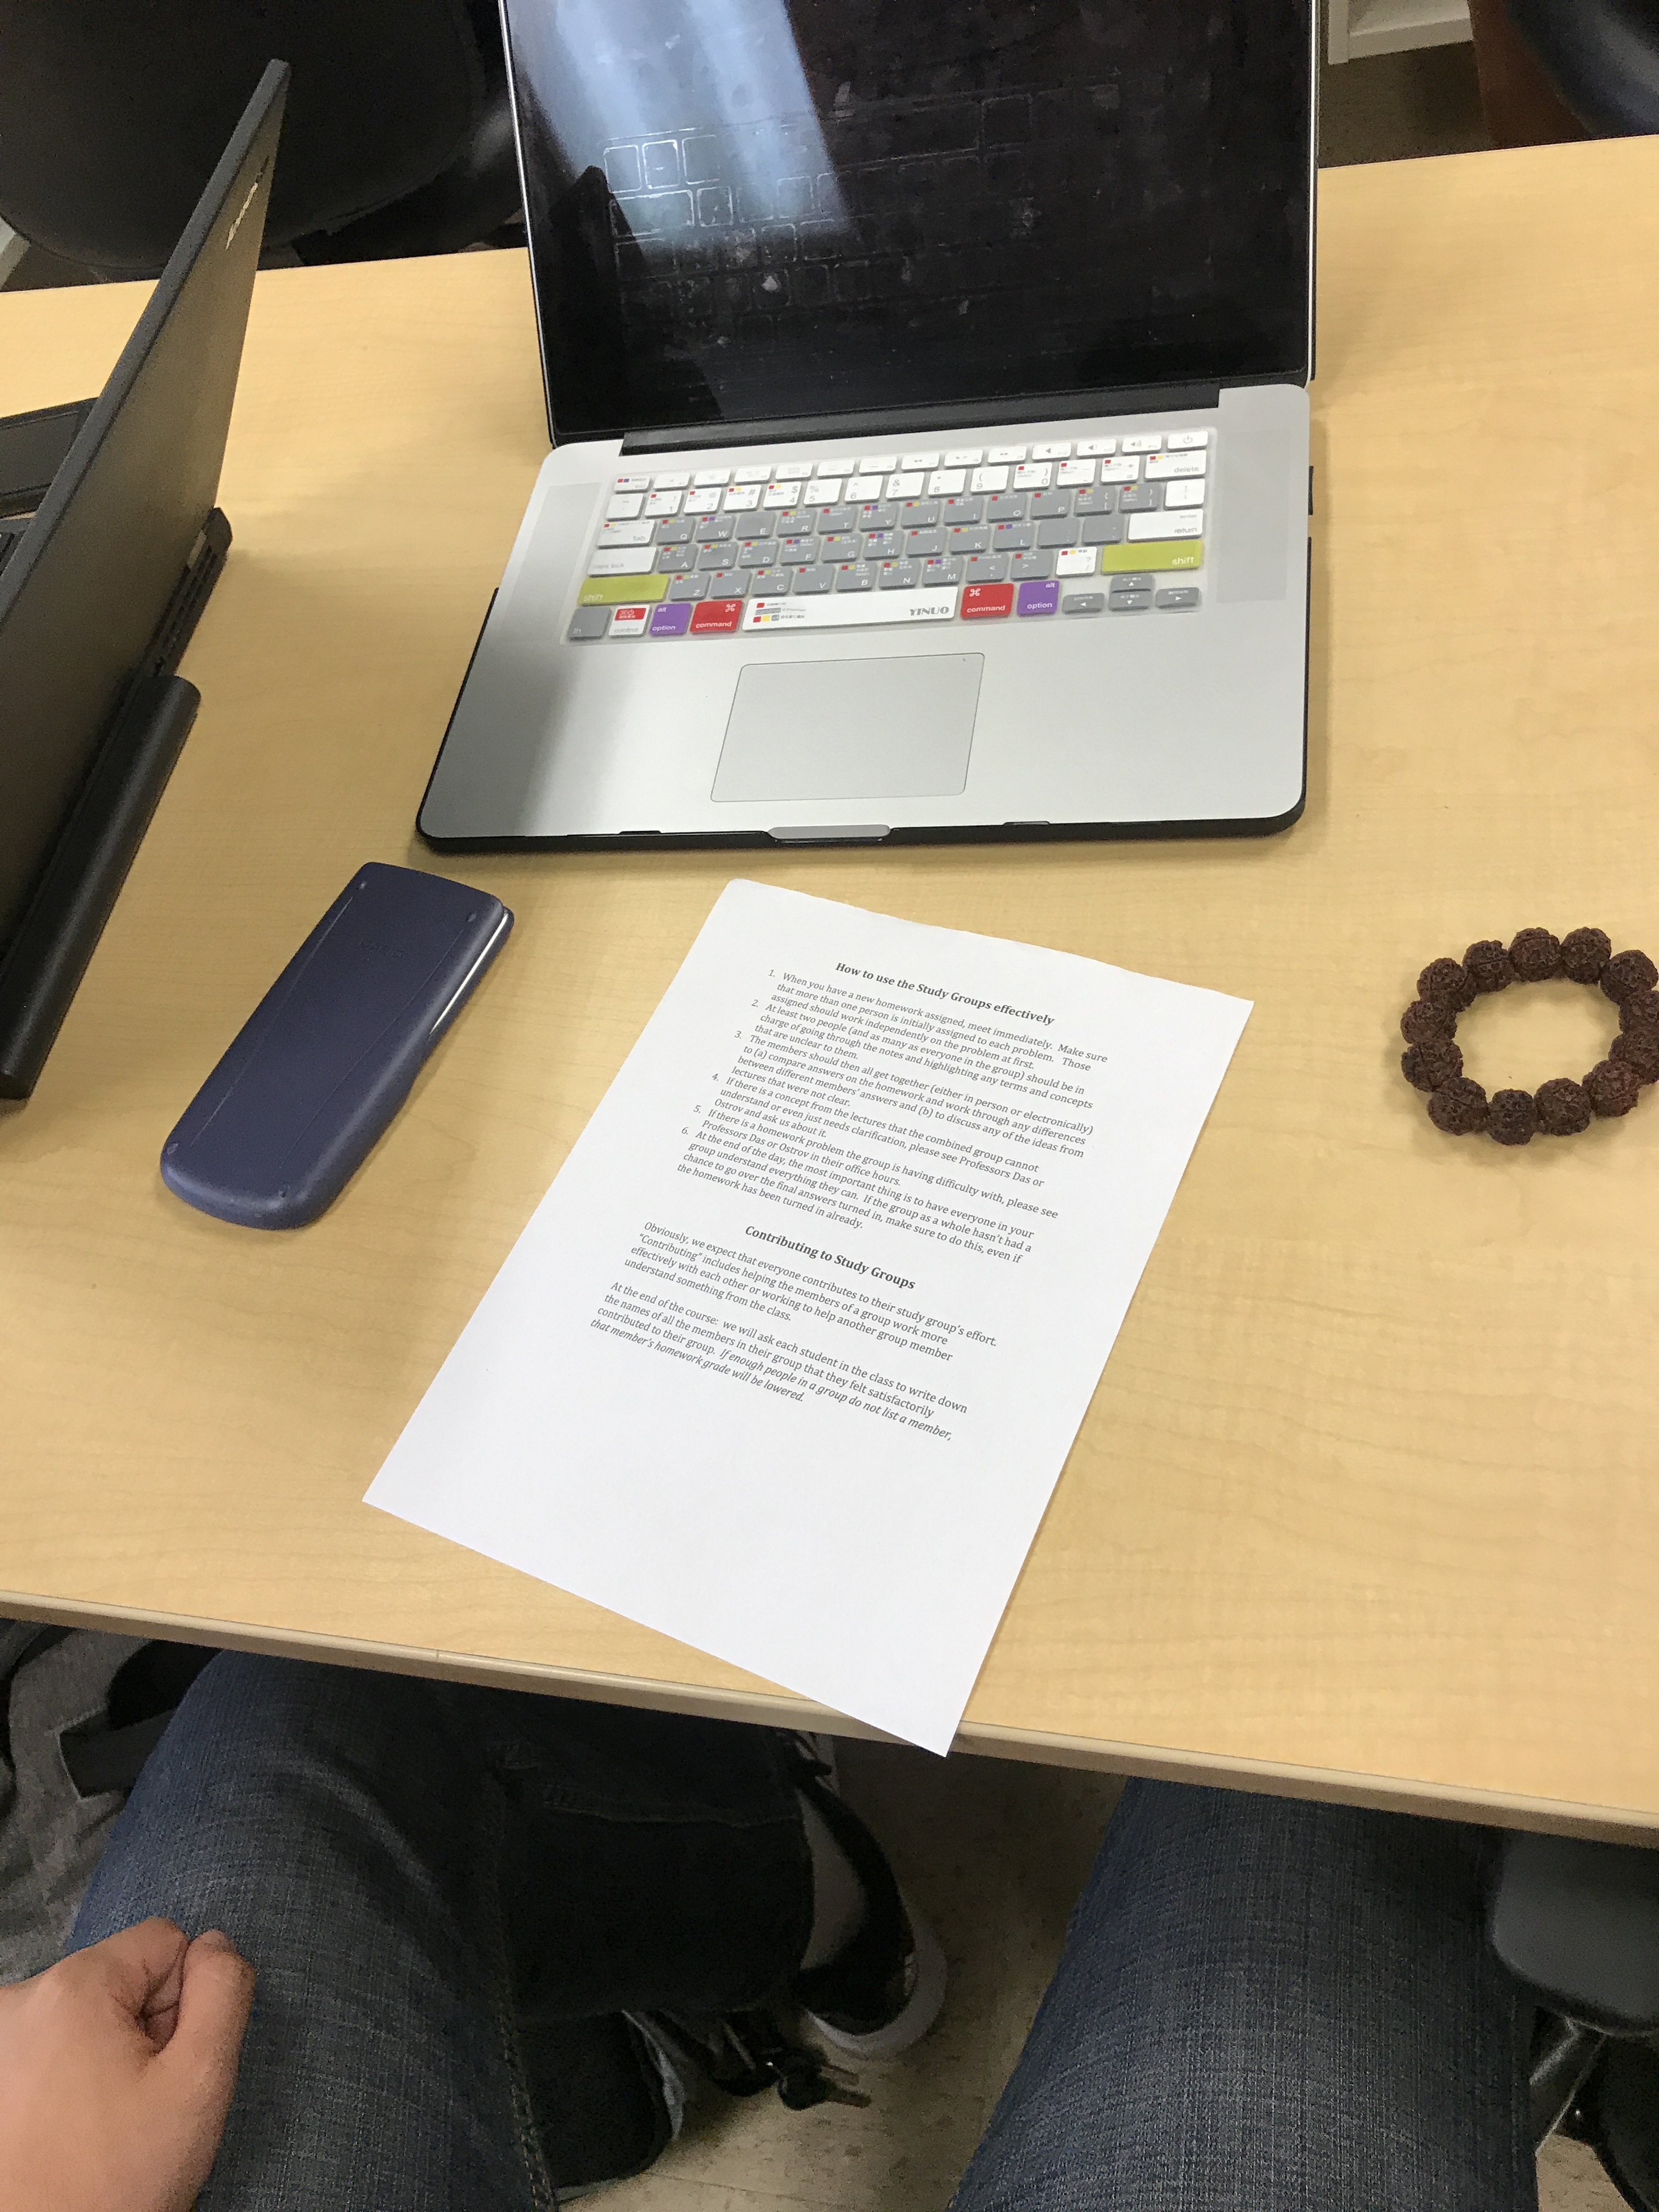
\includegraphics[width=.4\linewidth]{similar1.JPG}\hfill
	  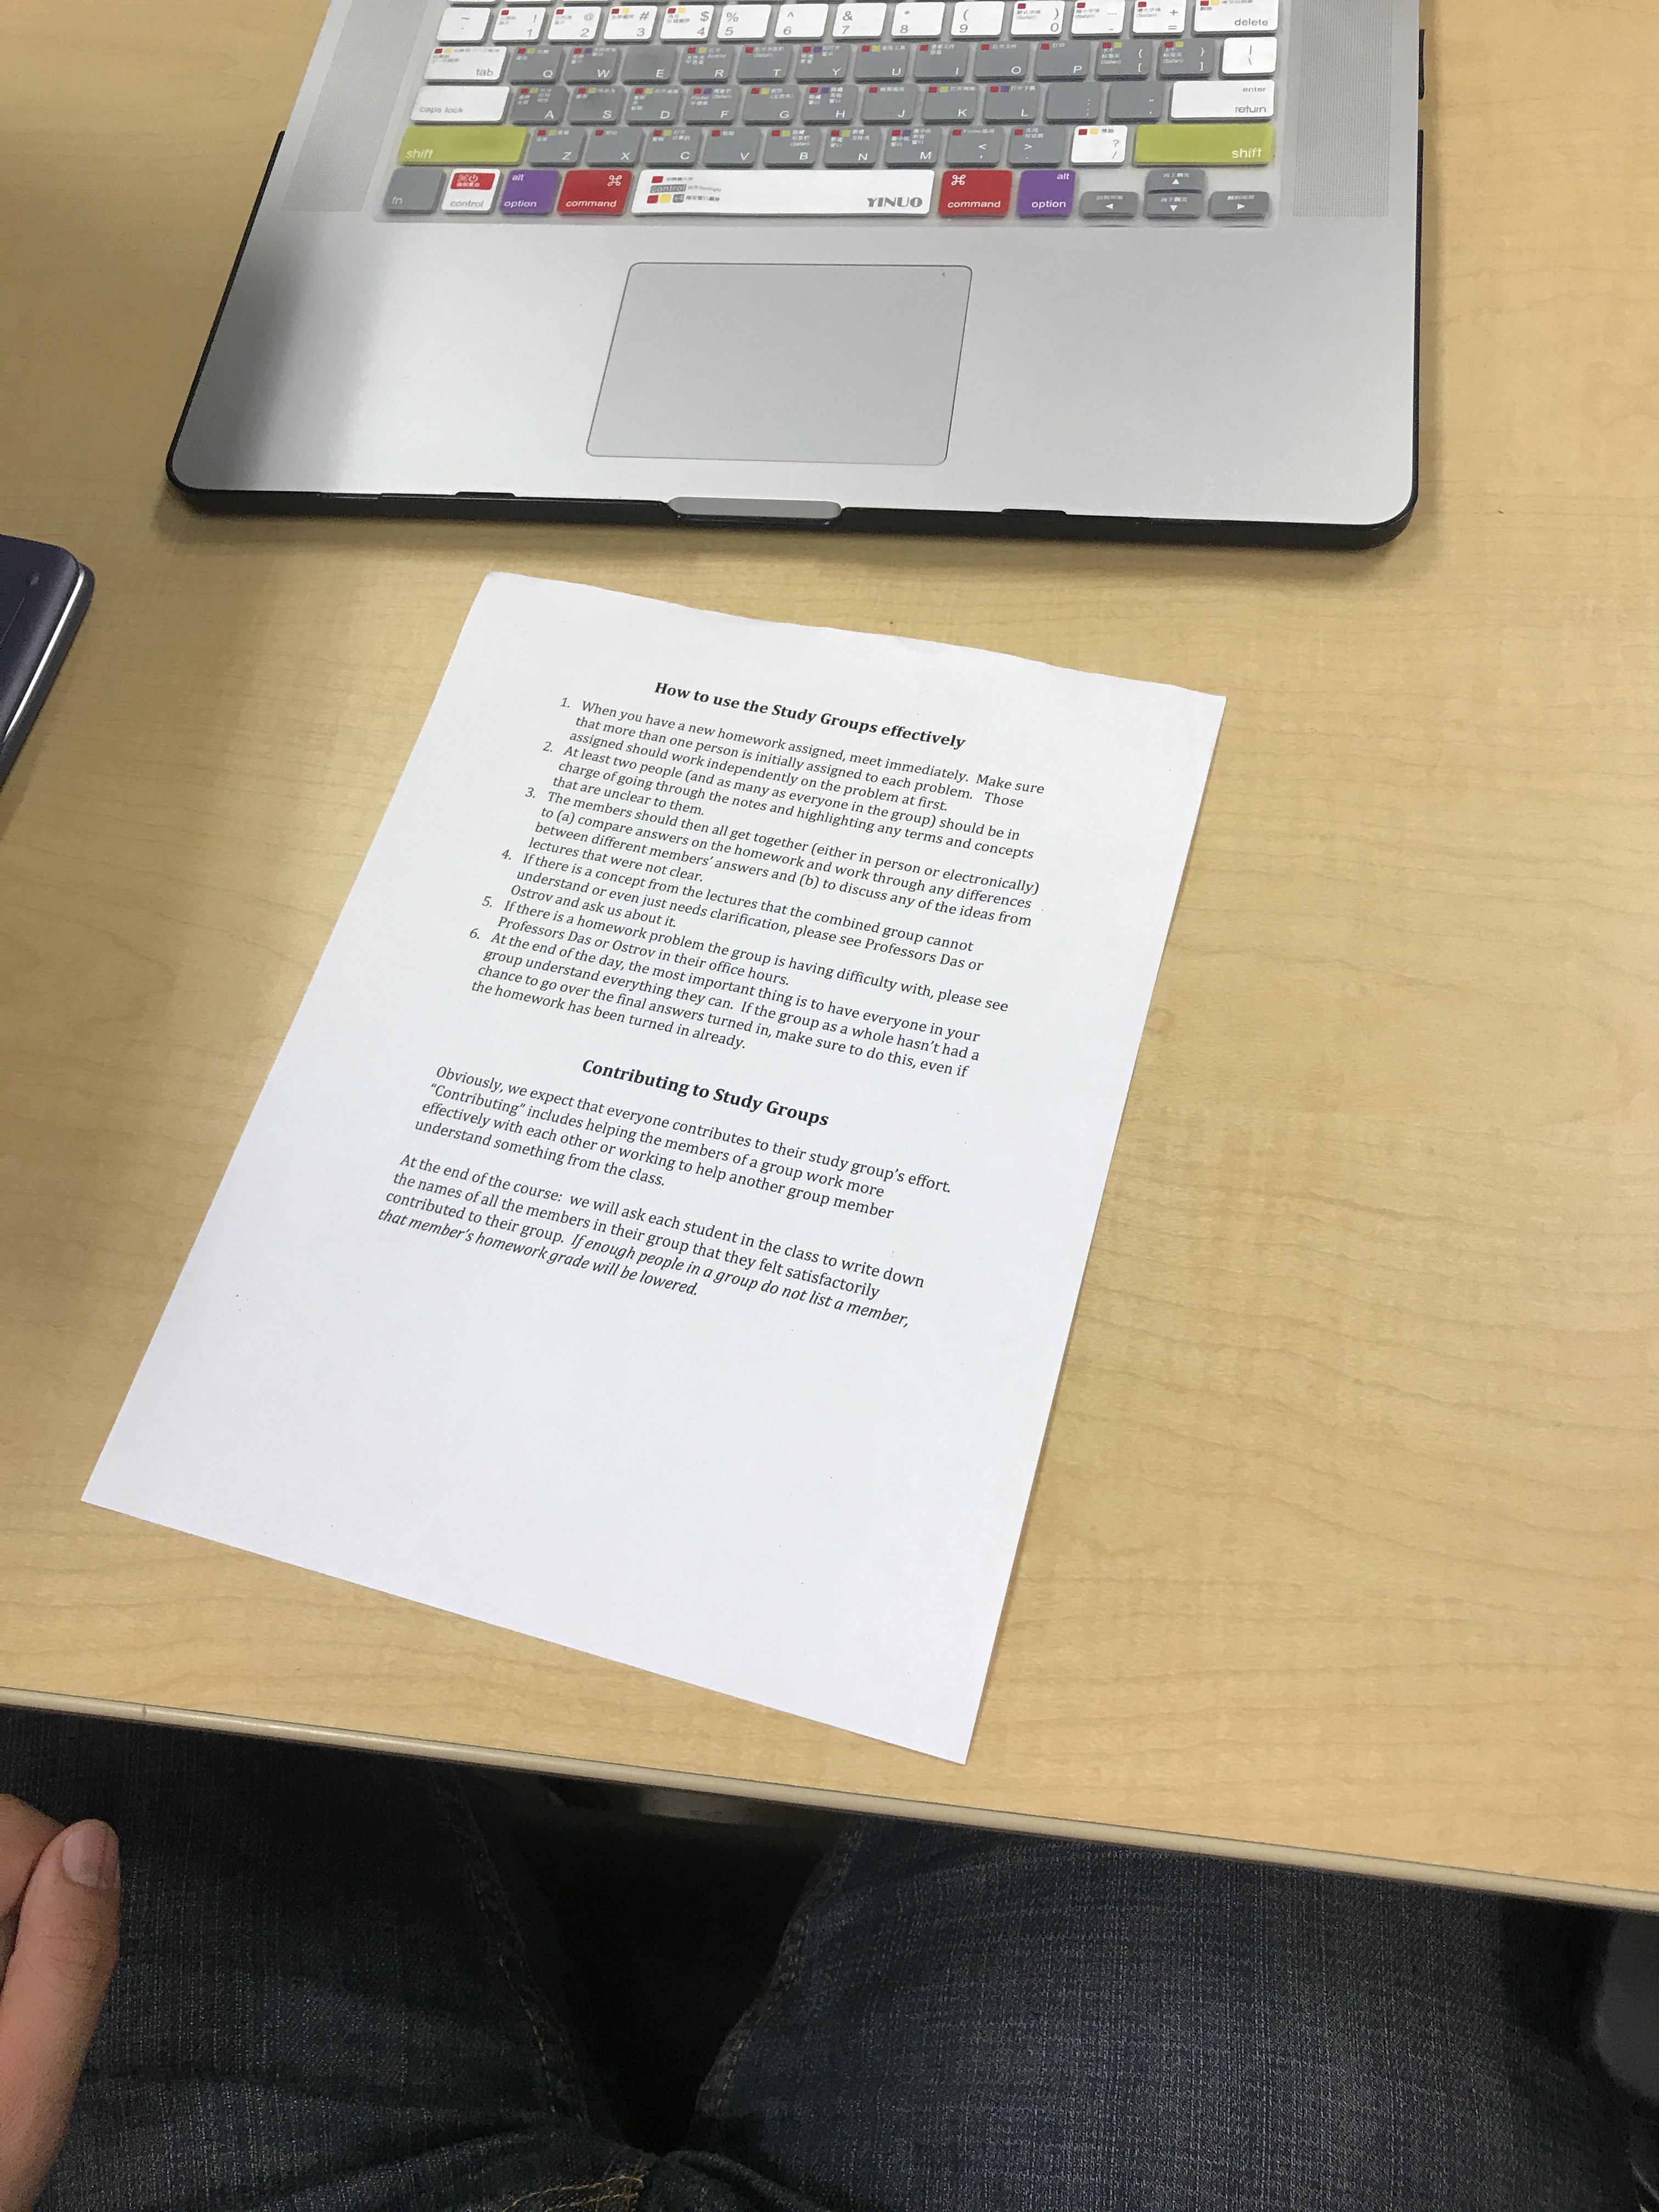
\includegraphics[width=.4\linewidth]{similar2.JPG}
  \end{subfigure}\par\medskip  
  
    \caption{Similar Images}
	\label{similarImages}
\end{figure}

\subsection{Image Processing}
\begin{figure}
	\centering
    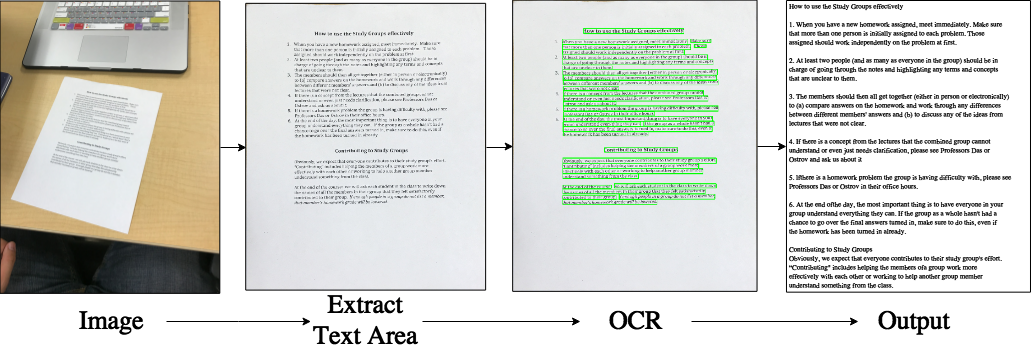
\includegraphics[scale = 0.4]{ImageProcess.png}
    
    \caption{Image Process Flow}
	\label{imageProcessFlow}
\end{figure}
When the image passed the blurriness test and the similarity test, the system will try to detect the text area in the image and extract the text area. The extracted text area is then sent to the Tesseract Optical Character Recognition (OCR) Engine to convert the image to computer encoded characters. (see Figure~\ref{imageProcessFlow})

\subsubsection{Text Area Extraction}
\begin{figure}
	\centering
    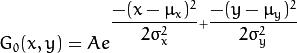
\includegraphics[scale = 1]{gaussianBlur.png}
    
    \caption{Gaussian Blur Equation}
	\label{GaussianBlurEquation}
\end{figure}
To extract the text area, a copy of the image is first blurred (5x5 Gaussian Blur is used in implementation \cite{gaussianBlur}) to detect the edges in the image (Canny Edge Detection is used in implementation \cite{canny}). From the edges of the image, contours are then collected \cite{contours} from the connected edges and sorted in descending order based on their area.

From the list of sorted contours, the biggest contour that can be approximated to a quadrilateral is identified as the text area. The text area is then applied with a perspective transformation to convert the text area to a rectangle	 as if the document is scanned. This increases the accuracy of the result from Tesseract OCR Engine. 

\subsubsection{Text Detection}
The transformed text area is processed by the Tesseract OCR Engine to identify the bounding boxes of the text in the image and convert the image to computer encoded characters. The computer-encoded characters are then processed to extract key features and feedback to the user.

\section{Text Summarization}
In order to provide users with a summary of the extracted text we use an algorithm called Term Frequency-Inverse Document Frequency \cite{tfidf} ~(TFIDF). The reason why TFIDF was chosen for our text summary is because it's one of the more popular and well known term-weighting schemes, it's easy to implement, and once it's set up it is computationally fast.

The goals of TFIDF are to obtain statistically important keywords from a text article. 

It does this by giving each word in the target document a score based on two statistics, the word frequency and the inverse document frequency.

The word frequency is simply the number of times the word appears in the target document and the inverse document frequency is calculated by taking the log of the total number of documents in a text corpus (described below) divided by the number of documents that the word appears in.

The final score for each word is calculated as follows: 

	\forceindent $tf(t, d) * idf(t, D)$  

where,

	\forceindent $tf(t, d) = 1$ if term $t$	is in Document $d$ else it's $0$

	\forceindent $idf(t, D) = log(\frac{N}{|d \in D : t \in d|}$

where,

	\forceindent $N$ is the number of documents in the corpus $N = |D|$

	\forceindent ${|d \in D : t \in d|}$: number of documents where the term $t$ appears.

The rationale behind the TFIDF algorithm is to reduce the importance of words that appear often yet have no overall significance. Examples of such words are: the, and, is, etc.


The corpus of documents are gathered in the news domain so that our text summarization is inline with the domain of PRAHVI functional requirements. Our strategy was to build our corpus by scraping the top online news repositories for all of there news articles. 

We took the 50 top online news websites. We used a Python library called Newspaper to gather the content of every article currently exists on the site.

Once our corpus was collected we precomputed the inverse document frequencies for each term in our corpus.
